\documentclass[10pt]{report}
%\usepackage[margin=.5in,landscape]{geometry}
\usepackage[margin=.5in]{geometry}
\usepackage{tikz}

\begin{document}
  \begin{center}
	%\includegraphics[width=.15\textwidth]{PSSC_Logo.png}\\
   {\bf \Large 5.2 ~ ~ ~ Regression ~ ~ ~ 10/15/2020}\\[.5in]
 \end{center}

\setcounter{chapter}{5}
\setcounter{section}{1}

\section{Getting Least Squares Line of Best Fit} % (fold)
\label{}
\subsection{From Calculator}
	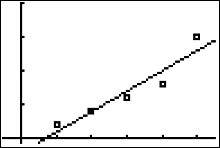
\includegraphics[width=.15\textwidth]{img/5_scat}

\subsection{From Summary Statistics} % (fold)
\label{sub:from_summary_statistics}
{\bf Formulas} (given): $\hat{y} = a + bx$\quad\quad$b = r\frac{s_y}{s_x}$\quad\quad$a=\bar{y}-b\bar{x}$\\[.2in]
{\bf Descriptive Statistics}: x, y\\  
\verb|Variable  N  N*   Mean  SE Mean  StDev  Minimum     Q1  Median     Q3  Maximum|\\
\verb|x         5   0  3.000    0.707  1.581    1.000  1.500   3.000  4.500    5.000|\\
\verb|y         5   0   7.00     2.24   5.00     2.00   3.00    6.00  11.50    15.00|\\[.1in]
{\bf Correlations}: x, y \\
\verb|Pearson correlation of x and y = 0.949|\\
\verb|P-Value = 0.014|\\[.5in]

% subsection from_summary_statistics (end)

\subsection{From Output} % (fold)
\label{sub:from_output}
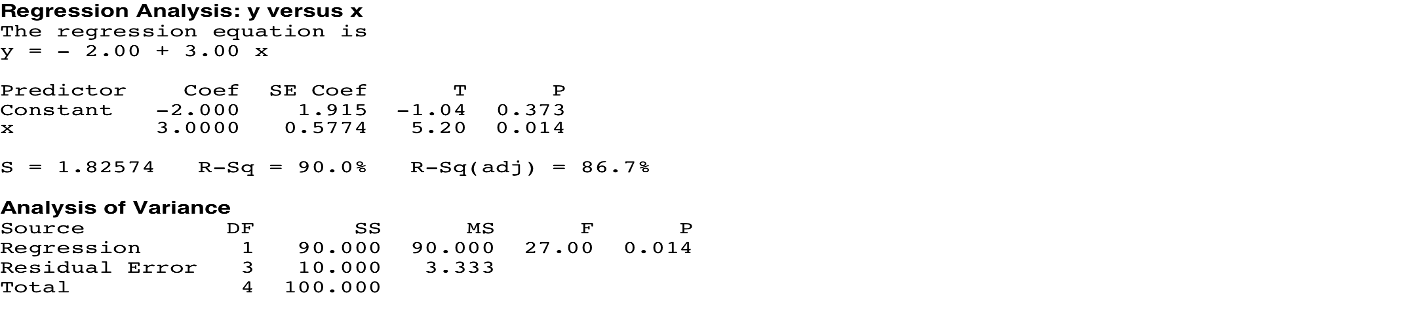
\includegraphics[width=1\textwidth]{img/5_RegOut}\\[.25in]

\subsection{Interpretation} % (fold)
\label{sub:interpretation}
\subsubsection{Slope}
Slope represents the  \textbf{predicted} change in response associated with each unit increase in the explanatory variable, \textbf{on average}.\\[.25in]
\subsubsection{Y-Intercept} 
Y-intercept is the predicted value when the explanatory $(x)$ is 0. [Often the y-intercept is useless.]
% subsection interpretation (end)

\end{document}